\documentclass[letterpaper,12pt]{article}
\pagestyle{empty}
\raggedbottom
\raggedright

\usepackage[svgnames]{xcolor}	% For Defining Color
\usepackage{framed}		% For custom Section Heading
\usepackage{times}		% For Handling Title Font Size etc. 
\usepackage{graphicx}		% For includegraphics
\usepackage{multirow} 		% For title table
\usepackage{enumerate}		% For Enumeration
\title{ArjunSadananda-Resume}

%----------------------Margin setup-------------------------%
% Defining Paper Dimensions
\setlength{\paperheight}{11in}
\setlength{\paperwidth}{8.5in}
% Defining Text Space
\setlength{\textheight}{10.5in}
\setlength{\textwidth}{7in}
% Defining Text Margins
\setlength{\topmargin}{-1.1in}
\setlength{\evensidemargin}{-0.25in}
\setlength{\oddsidemargin}{-0.25in}
% Width of border outside of title bars
\newlength{\borderthickness}
\setlength{\borderthickness}{3pt} 

%--------------------Define Colors--------------------------%
\definecolor{bgColor}{gray}{0.98}	% Page Background Color
\pagecolor{bgColor}

\definecolor{shadecolor}{gray}{0.75}	% Used by \framebox
\definecolor{section_bg}{gray}{0.93}	% Used by \fcolorbox

%-------Defining Custom command: For Section Heading----------%
\newcommand{\sectionheading}[1]{
	\vspace{8pt}
		\parbox{\textwidth}{\setlength{\FrameSep}{\borderthickness}
		\begin{shaded}
			\setlength{\fboxsep}{0pt}
			\framebox[\textwidth][l]
				{\setlength{\fboxsep}{4pt}
					\fcolorbox{section_bg}{section_bg}	{\textup
											{\rmfamily
												{\mbox{~}\makebox[6.65in][l]
													{\LARGE #1} \vphantom{p\^{E}}
												}
											}
										}
				}
		\end{shaded}
		}
	}

\begin{document}

	% Insert Picture and Title
	\begin{tabular}{p{2.2in} p{4.5in}}
  		\multirow{4}{*}{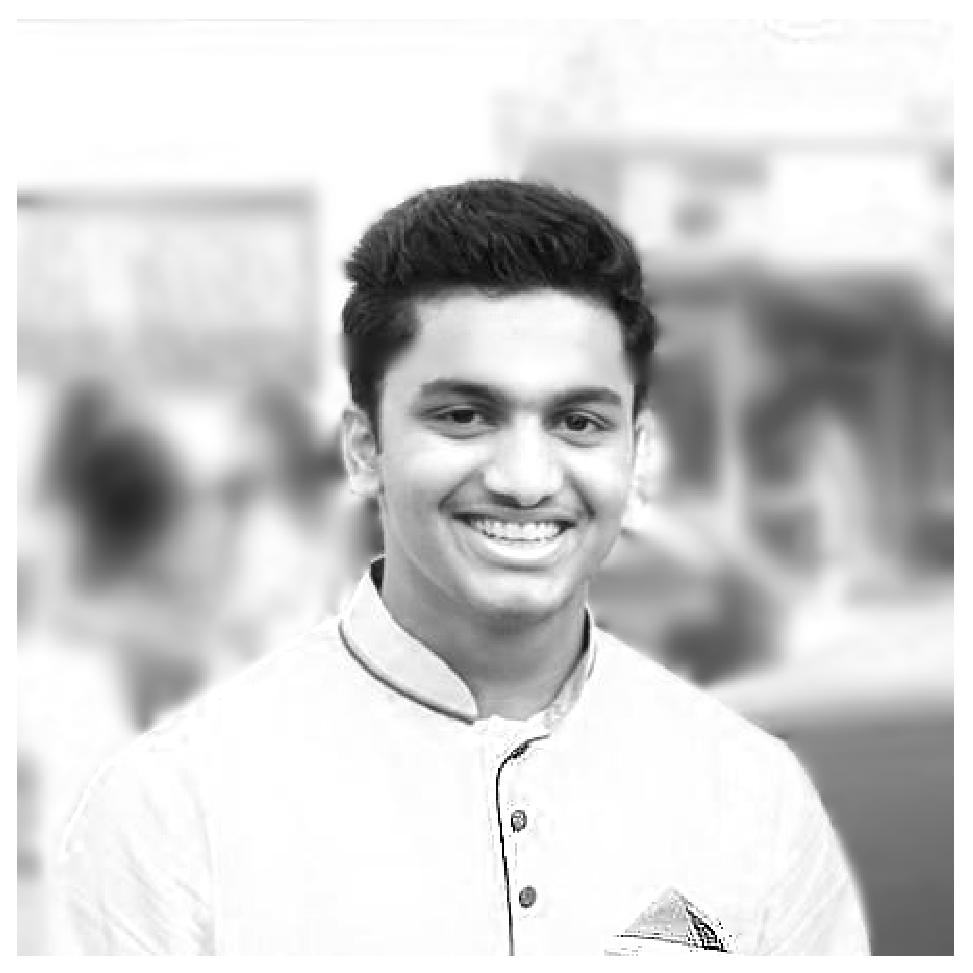
\includegraphics[scale=0.3]{photo}}\\
  	
		& \textsf{\textsc{\fontsize{37}{10} \selectfont Arjun Sadananda}}\\ % Small Caps
		& \\  		
		& National Institute of Technology Karnataka, Surathkal  \\
		& Manglore-575025 \\
		& Karnataka\\
  		& Email  : arjun.sadananda@gmail.com \\
		& Contact: +91 9980402770
		
	\end{tabular}
	\vspace{0in}
	
	% Career Objective
	\sectionheading{Career Objective}
	\begin{center}
		My career goal is to design and program robots for a better future.\\
		My interest lies in Computer Vision, Motion Planning, Control Systems, \\ 
		Mechanical design CAD|CAM and everthing robotics.
	\end{center}

	% Education
	\sectionheading{Education}
	\begin{center}
		\begin{tabular}{ |p{5in}|p{.8in}| } 
			\hline
			\hspace{.1in} \textbf{National Institute of Technology Karnataka, Surathkal} & \hspace{.1in} \textbf{2015-19 } \\ 
			\hspace{.1in} \textit{Bachelors in Mechanical Engineering}  &\\
			\hspace{.1in} Coursework includes Manufacturing Technologies, CAE, Analysis &\\
			\hspace{.1in} and Synthesis of Machines, Machine Drawing. &\\
			\hline
			\hspace{.1in} \textbf{Indian Educational School, Kuwait} & \hspace{.01in} \textbf{2009-2015 } \\ 
			\hspace{.1in} \textit{High School Science and Computer Science}  &\\
			\hspace{.1in} Kuwait Topper in Class 12 CBSE Computer Science &\\
			\hline
		\end{tabular}
	\end{center}

	% Projects and Achievements
	\sectionheading{Projects/Achievements}
	\begin{enumerate}[I]
		\item eYantra Robotics Competition- IIT Bombay: Third Position -March 2017\\
			- Focus on Path Planning, PID Control on Differential Drive robot- FireBird and Image Processing\\
			- Found out of the box solutions to problems like parallax error in robot position 
			estimation using camera, Mechanical Design of robotic Arm/Grabber, 
		\item Automata: Winning Team Leader and lead programmer -October 2016\\
			Image Processing(Over-Head Camera) and PID Control based robotics
			competition, conducted during Engineer(NITK) one of the largest Tech
			Fest in South India.
		\item Brain Computer Interface: For Robotic Arm - In Progress\\
			Working Under CSD Labs NITK
		\item Robotic Wooden Arm: Controlled using Arduino (Hobby Project)
	\end{enumerate}

	\pagebreak

	% Training and Internships
	\sectionheading{Training and Internships}
	\renewcommand{\labelitemi}{$\diamond$}
	\begin{itemize}
		\item International Conference on Control Systems- APCOSEC 2016\\
			Interacted with world renowned Systems Engineers and Graduates behind\\
			Student Satellites. Industrial Visit to ISRO Satellite Center.\\
		\item Certified Online Courses related to Robotics:
		\begin{itemize}
			\item Control Theory for Mobile Robots – Coursera GeorgiaTech
			\item Machine Learning- Coursera Stanford
			\item Applied Computer Science with Android – Google (in NITK Campus)
		\end{itemize}
	\end{itemize}

	% Technical Skills
	\sectionheading{Technical Skills}
	\begin{tabular}{ p{2in} p{2in}}
		OpenCV			& * * * * * * - - - - \\
		Matlab/ Octave		& * * * * * - - - - - \\
		Arduino, Raspberry Pi	& * * * * * * * - - - \\
		Android Studio		& * * * * * - - - - - \\
		Embedded C		& * * * * * - - - - - \\
		CATIA			& * * * * * * - - - - \\
		PLC (Ladder Logic)	& * * * * * - - - - - \\
	\end{tabular}

	% Soft Skills
	\sectionheading{Soft Skills}
	\begin{enumerate}[I]
		\item Leadership
		\item Public Speaking
		\item Debating
		\item Photo, Music and Video Editing
	\end{enumerate}

	% Co-Curricular Activities
	\sectionheading{Co-Curricular Activities}
	\begin{enumerate}[I]
		\item IEEE Student Member (2015-2016)
		\item Student Council Member, NITK (2015-2016)
		\item Deputy Head Boy, Student Council, Indian Educational School, Kuwait.
		\item Iken Scientifica: Kuwait Runner Up\\
		A national level science competition to establish a connection between curricular knowledge and practical application
	\end{enumerate}

	\pagebreak

	% Extra Curricular Activities
	\sectionheading{Extra Curricular Activities}
	\begin{itemize}
		\item Co-Founded TheGreenBrigade, Presently under NSS, NITK\\
			Organized Campus Clean Up Drive inspired by Swachh Bharat Abhiyan
		\item National Cadet Corps (August 2015 – November 2016)
	\end{itemize}

	% Languages
	\sectionheading{Languages}
	
	\begin{tabular}{p{2in} p{2in}}
		 English	& * * * * * * * * * - \\
		 Hindi		& * * * * * * * * - - \\
		 C/C++		& * * * * * * * * - - \\
		 Java		& * * * * * - - - - - \\
		 Python		& * * * * * - - - - - \\
	\end{tabular}

	% Research Publication
	\sectionheading{Research Publications}
	\begin{enumerate}[(i)]
		\item Hopefully, Coming Soon...
	\end{enumerate}	
	
\end{document}
